With our background in both machine learning and \todo{medical background} we can now look at how we want to solve the problems associated with setting up a system for medical diagnosis.  
We will first look at the language and packages used in the creation of this thesis. We will go in depth into the reasoning behind why we chose the tools and packages that became the foundation of the programs. 

Then we will look at the setup of the complete program. Here we will go in-depth into both the different preprocessing algorithms, and take a look at the transfer learning network used during classifying.
\section{Birds eye view (Chapter removed when written)}
\todo{we have 2 hps, put them here.}

\noindent
\begin{hyp} \label{hyp:a}
When classifying images, we will get the best result when we have images with the least amount of sparse information. 
Hence by removing areas with sparse information,
we will see an increase in classification performance compared to not removing areas.
\end{hyp}

\noindent
and

\noindent 
\begin{hyp} \label{hyp:b}
When training a classifier, we will get a higher
mode of generalisation of our results when removing the dataset
specific artefacts compared to not removing artefacts.
\end{hyp}
\vspace{5px}

\section{Libraries} 
In this chapter, we will discuss the foundation of our code, important external libraries, and the setup and execution of our project.  
We will first discuss the programming language in question, give insight into the reasoning behind it. Then we will look into the framework used for machine learning, and in detail how it implemented in our programming language. Lastly, we will look into the wrapper we use to get a higher level of abstraction over our code, together with custom wrapper functions that are used by our wrapper. 

\subsection{Python}
When doing machine learning, the most popular languages, in no particular order, are Python, Java, R, C++, and C \todo{cite}. Some of these languages, like C and C++, are chosen for their speed, which is often a significant factor in Machine learning. Other languages, like R, is chosen because of its integration into the scientific community long before machine learning became a trend. The last group, consisting of Java and Python has gained popularity because of its already big user base and user-friendliness. Python is also the winner when it comes to machine learning because of, like R, its integration into the scientific community. 
Right now Python is the leading language for machine learning. Driven by this, there is considerable focus into making it faster, to compete with already fast languages, like the C family. 

Python is an interpreted, high-level, general-purpose programming language created in 1991.   It, like many other modern languages, is object-oriented and supports functional programming. 

Mainly because of the excellent support when it comes to machine learning, and the general "easy to use and no compiling" we have chosen python as the base for our code in this thesis. 



\subsection{Tensorflow}
Arguably the biggest reason for the success of machine learning in python lies in Tensorflow.\todo{cite} Tensorflow is a machine learning package developed by Google in \todo{year} and has since then become the leading framework for machine learning worldwide \todo{cote}.  
Tensorflow is in use by companies like AMD, Nvidia, eBay and Snapchat. 


\todo{something about projects with python, and how may uses}

Tensorflow is today a multi-language tool, but it had its origin in python. It is just in later years that other languages have gotten tensorflow support.  
The data flows through a graph network, where the objects in the graph describe the mathematical operations used in the machine learning, and the edges between graphs are the multidimensional arrays storing the weights associated with the operation in question. The name Tensorflow is a combination of the flow we experience during calculation and the tensors between the mathematical operations. 

As stated, Python, and subsequently machine learning in Python, would be much slower than a counterpart in C. Because of this, Tensorflow works as a layer of abstraction to code running in the C language. 
 
\todo{cpu vs gpu}
\todo{, CNTK, or Theano}



\subsection{Keras}
One of the least attractive things with tensorflow is its unnecessary complexity.  Even though Tensorflow offers more abstraction compared to running the code in pure C, the Tensorflow library can be unnecessarily complex.
As a result of this, many external libraries try to simplify many of the complexities that accompany tensorflow. 
Libraries like TFlearn was made as a modular and transparent deep learning library on top of tensorflow. It gives a higher-level API to Tensoflow to reduce complexity and speed up experiments. \todo{cite TFLEARN}
The most successful library for on top of Tensorflow is Keras \todo{cite keras}. 
Just as TFlearn, Keras is a high-level package written in python. It is capable of running on top of TensorFlow, CNTK, or Theano, which is the tree most popular machine learning libraries at this time. 
From their website they state that their four goals when creating Kears were:
\textbf{User friendliness. }\\
\textbf{Modularity. }\\
\textbf{Easy extensibility.}\\ 
\textbf{Work with Python. }\\

One of the core elements of Keras that makes it a better choice than just running, for instance, Tensorflow, is the concept of a model. A model in Keras is a way to organise the layers of the network in a more organised way, giving a better understanding of how the network is set up, and how each layer type contributes to the graph. \todo{more}

This thesis relies on Keras as a wrapper for tensorflow. As stated, the use of models and the simplicity of the language makes it an excellent choice of such a large project. Also, Keras has good support for convolutional operations which is the most used methods when managing images. Keras also has the most popular pretrained convolutional neural network models available in its package. \textit{Since one of our primary goal is to see how well our datasets generalise to the real world, transfer-learning will be a great tool to forgo unnecessary training}





    
\section{Custom functions for Keras, tensorflow and python}
\subsection{CWFC layer}
A problem often encountered when working with autoencoders which are not undercomplete is the fact that they learn to represent the data flawlessly. \cite{OvercompleteAE} 
When this problem arises, the network does not learn the fundamental features that define the dataset and instead passes the signal through the network without any consideration of the input data.
This flaw will often defeat the purpose of the algorithm, so data scientists often put in safeguards, like undercompleteness or regulisers, to combat this lack of feature learning. 
This problem extends to other types of generator networks where there are not sufficient compression or regularisation in the layers of the network.
Even though this problem often is solved by compressing the network into a space that can not contain the information exactly, the network does not always learn the features that define the network. 

We propose a custom ``channel-wise fully-connected layer'' in Keras to help with the problem of correctly learning features. This layer is based on the work done by Pathak et al. in their paper on content encoders\cite{Pathak_2016}.

The channel wise fully connected layer is primarily used in the GAN to transfer information within each feature map, without using convolutions to do it. As we recall, fully connected layers are often not suitable because of the large size of the weight layer associated with it. This layer is essentially a fully connected layer with groups, where the goal is to propagate the information within each feature map.
Given the latent space of $n \times n$ with $m$ feature maps, by not connecting the feature maps together in the fully connected layer we achieve a parameter reduction from $m^2n^4$ to $mn^4$ (ignoring bias terms) \cite{Pathak_2016}

With the ``channel-wise fully-connected layer'' the network can learn features from the entirety of the image, and not just local regions as it would with just convolutions. 

Listing \ref{listing:CWDense} shows the source code used for the channel-wise fully-connected layer.

\begin{listing}[h]
\begin{minted}[fontsize=\footnotesize]{python}
from keras.engine.topology import Layer
import keras.backend as K

class CWDense(Layer):
    def __init__(self, **kwargs):
        super(CWDense, self).__init__(**kwargs)
    
    def build(self,input_shape):
        _, self.width, self.height, self.n_feat_map = input_shape
        self.kernel = self.add_weight("CWDense",
                                        shape=(self.n_feat_map,
                                        self.width*self.height,
                                        self.width*self.height),
                                        initializer='glorot_uniform',
                                        trainable=True)        
        super(CWDense, self).build(input_shape)

    def call(self, x):
        x = tf.reshape( x, [-1, self.width*self.height, self.n_feat_map] )
        x = tf.transpose( x, [2,0,1] )

        x = K.dot(x,self.kernel)

        x = tf.transpose(x, [1,2,0])
        x = tf.reshape( x, [-1, self.height, self.width, self.n_feat_map] )
        return x

\end{minted}
\caption{The channel-wise fully-connected layer source code}
\label{listing:CWDense}
\end{listing}

\subsection{Subpixel}
When working with the generative adversarial network, we wanted to achieve more realistic representations at a reasonable image size. 
Making large scale images in generative adversarial networks has been a challenge that has only recently been cracked. \cite{DBLP:journals/corr/DentonCSF15} \cite{DBLP:journals/corr/abs-1809-11096}
As an early measure to fix this problem, we experimented with the use of a Sub-pixel layer as presented by Shi et al.~\cite{DBLP:journals/corr/ShiCHTABRW16} to give a more realistic output compared to just a standard conv-tanh layer.

\begin{figure}[h]
\centering
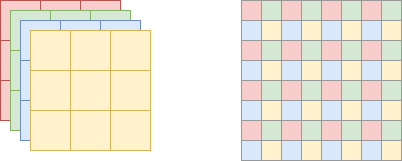
\includegraphics[scale=0.8]{methodology/figures/SubPixel.png}
\caption{How the layers in the sub pixel layer is stacked. Recreated from the SubPixel paper by Shi et al.~\cite{DBLP:journals/corr/ShiCHTABRW16}}
\label{fig:SubPixel}
\end{figure}






%\subsection{Spectral conv?}
\subsection{Masklaod}
\subsection{Self attention}
There are features in the images that are more important than others. One of the things we often want to preserve when we recreate images are hard edges. To get a semantically meaningful image,  we often want to differentiate between background and the mucosa. 
To see if the network can learn the features needed we are Introducing the Self Attention layer to help with this. 


\begin{listing}[h]
\begin{minted}[fontsize=\footnotesize]{python}
class Attention(Layer): 
    def __init__(self, filters, **kwargs):
        self.filters = filters
        super(Attention, self).__init__(**kwargs)

    def build(self,filters):
        self.kernelf = self.add_weight(name='kernelf', 
                                      shape=(1,1,self.filters,self.filters),
                                      initializer='uniform',trainable=True)
        self.kernelg = self.add_weight(name='kernelg', 
                                      shape=(1,1,self.filters,self.filters),
                                      initializer='uniform',trainable=True)
        self.kernelh = self.add_weight(name='kernelh', 
                                      shape=(1,1,self.filters,self.filters),
                                      initializer='uniform',trainable=True)
        super(Attention, self).build(filters)

    def call(self, x):
        f = K.conv2d(x, self.kernelf, strides=1, padding="same")
        g = K.conv2d(x, self.kernelg, strides=1, padding="same")
        h = K.conv2d(x, self.kernelh, strides=1, padding="same")
        f = tf.transpose(f,perm=[0,1,2,3])
        i = f*g
        j = K.softmax(i)
        k = j*h
        return k

\end{minted}
\caption{The self attention layer source code}
\label{listing:Attention}
\end{listing}

\begin{figure}[h]
\centering
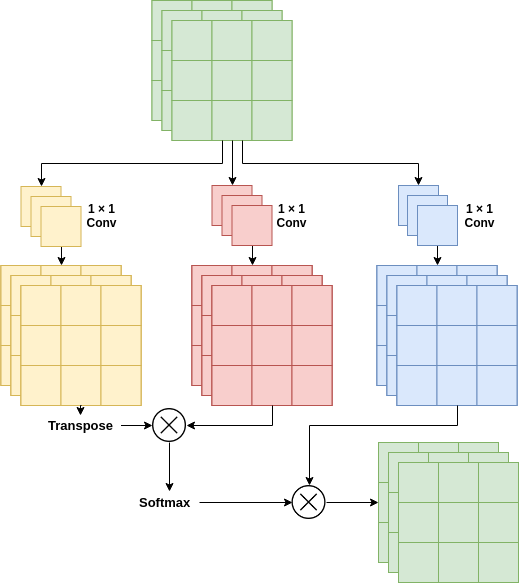
\includegraphics[scale=0.4]{methodology/figures/attention.png}
\caption{How the layers in the Self-Attention layer is stacked. Recreated from the Self-Attention  paper by Zhang et al.~\cite{DBLP:journals/corr/selfattention}}
\label{fig:Attention}
\end{figure}



\subsection{Masked loss}
A problem encountered for both the autoencoder and the GAN is what happens when the non-inpainted area gets too close to correct ground truth. 

\begin{itemize}
	\item 32 bit float
	\item small-small = really small
	\item really small squared is 0?
	\item zero gives us weird gradients?
	\item UNDERFLOW cuses bigass number
	\item Wromng calculation causes biggass number
\end{itemize}





\section{Stabilising the GAN}
Before we ended up with the model we used in the thesis we ran multiple experiments to make the generative adversarial network stable for training. 
In contrast to the autoencoder, the GAN does not use the ground truth as a reference point. Where the autoencoder always has a gradient based on the input data, the generator in the GAN gets its learning gradient from another network.

This lack of a ground truth gives the GAN many pitfalls that cause the training process to crash \footnote{Crashing is not the right word to use, but the result is the same: The learning process stops.}.


\paragraph{Normalise the inputs}
One of the first measures we did to prevent training collapse was to normalise the inputs. Instead of using images in the range 0 to 255 in pixel values we switched the values to  -1 to 1. 
Later, when the images were generated, we switched out the standard sigmoid output layer with a tanh output layer. As we wanted the output to be between -1 and 1, this was necessary, as the sigmoid only outputs between 0 and 1.

\paragraph{Using gaussian noise}
perhaps write about this



\paragraph{Normalising the batches}
One of the most significant challenges we encountered when training the adversarial network was the use of correct normalisation. 

The practice of training the discriminator with real and fake samples separately gave higher stability overall. 

The use of instance normalisation gave a better result compared to using batch normalisation. We believe this is contributed to the fact that the discriminator learned that the average pixel value was lower for the whole batch since the area inpainted had 0 as the pixel value.

The final model ended up not using batch or instance-normalisation. 



\paragraph{Avoiding sparse and vanishing gradients}
Most of the well-known networks use the ReLu\cite{Nair/2010/RLU/3104322.3104425} activation function \cite{DBLP:journals/corr/SimonyanZ14a} \cite{DBLP:journals/corr/SzegedyIV16} 
\cite{DBLP:journals/corr/HeZRS15}.
We saw the best result when we used non-sparse gradients during training. 
Instead of using ReLu we used the slightly modified LeakyReLu \cite{Maas2013RectifierNI}.

\todo{mention RReLu, but the number of parameters not worth it.}

In addition to trying to remove sparse gradients, we also wanted to address the problem with vanishing gradients during training. Given that we have fully saturated pixels (with the value of 1 or 255) and we have fully darkened pixels (with the value of -1 or 0) we, at the end of the experimentation phase, ended up removing the tanh layer. 
The removal of the tanh layer meant that the pixel values could be arbitrary on both positive and negative value, so we had to clip the value not to get an error at test time. 



\paragraph{Avoiding residual and inception layers}
When training the GAN experiments shows that the usage of both residual \cite{Rumelhart:1986:LIR:104279.104293} and inception \cite{DBLP:journals/corr/SzegedyLJSRAEVR14} models does note contribute to a good result when training the GAN.

Residual modules primary strength is that they always send the image/signal throughout the network in addition to the standard layers. Instead of the network needing to generate the whole image for each layer, the network instead adds or subtract from the original image for each layer.
This modification to the original image might seem reasonable when it comes to inpainting, but in reality, this does not work.  Given an image where we want to change only the inpainted area, the image is about 80\% unchanged. The network could focus on just filling in the inpainted area in theory, but in practice, the network tries to change the rest of the image in addition to the square. This incorrect inpainting gives us a generator that changes too much of the image and a discriminator that does not learn any important features since the input and output are relatively similar from the start.

Inception modules primary strength is the fact that the gradient can flow throughout the path most suited to the problem at hand.
We tested some training runs with inception modules, but the result was not impactful enough to continue to use this architecture.

From multiple training runs, it seems like just a straight forward encoder-decoder network for the generator yielded the best result. While the best result for the decoder was to use convolutions with stride do downsample the signal.

\todo{this might not be the right chapter for describing what layers are in the GAN, so please move}



\section{Design of the inpainting algorithms}
When inpainting we have multiple hypotheses we want to test to see how it affects the results. We first want to set up a platform where every dataset is made with the same parameters, except for the dataset-specific parameters that define the dataset. Based on the hardware limitations \todo{more?}

When generating the datasets, we use the Kvasir dataset as a base exclusively. When using only the Kvasir dataset, we have the CVC sets for testing. This selection of image source was made intentionally to have a fundamentally different test and training set, and the more differences between testing and training set the more of an indication of generalisation. 

%image used to be here

Figure \ref{fig:KvasirAnomaliesFIX} shows two different image types from the Kvasir dataset. 
Figure \ref{fig:LargeLeftBlack} shows the image class esophagitis. This image shows one of the main problems with the Kvasir dataset when it comes to dataset specific artefacts. In addition to the cut corners, we have an extra wide area to the left of the image containing non-relevant information like name, sex, and other comments. We can recall from chapter \todo{find where} that the area to the left does not contain any relevant information for the classification and subsequently can only give false information during classification. 
%Another example of dataset-specific artefacts is in the image (b). In this image, we have the same cut corners as in most colonoscopy images. However, we also have an additional green square in the bottom left corner.

\begin{figure}
     \centering
     \begin{subfigure}[b]{0.4\textwidth}
         \centering
         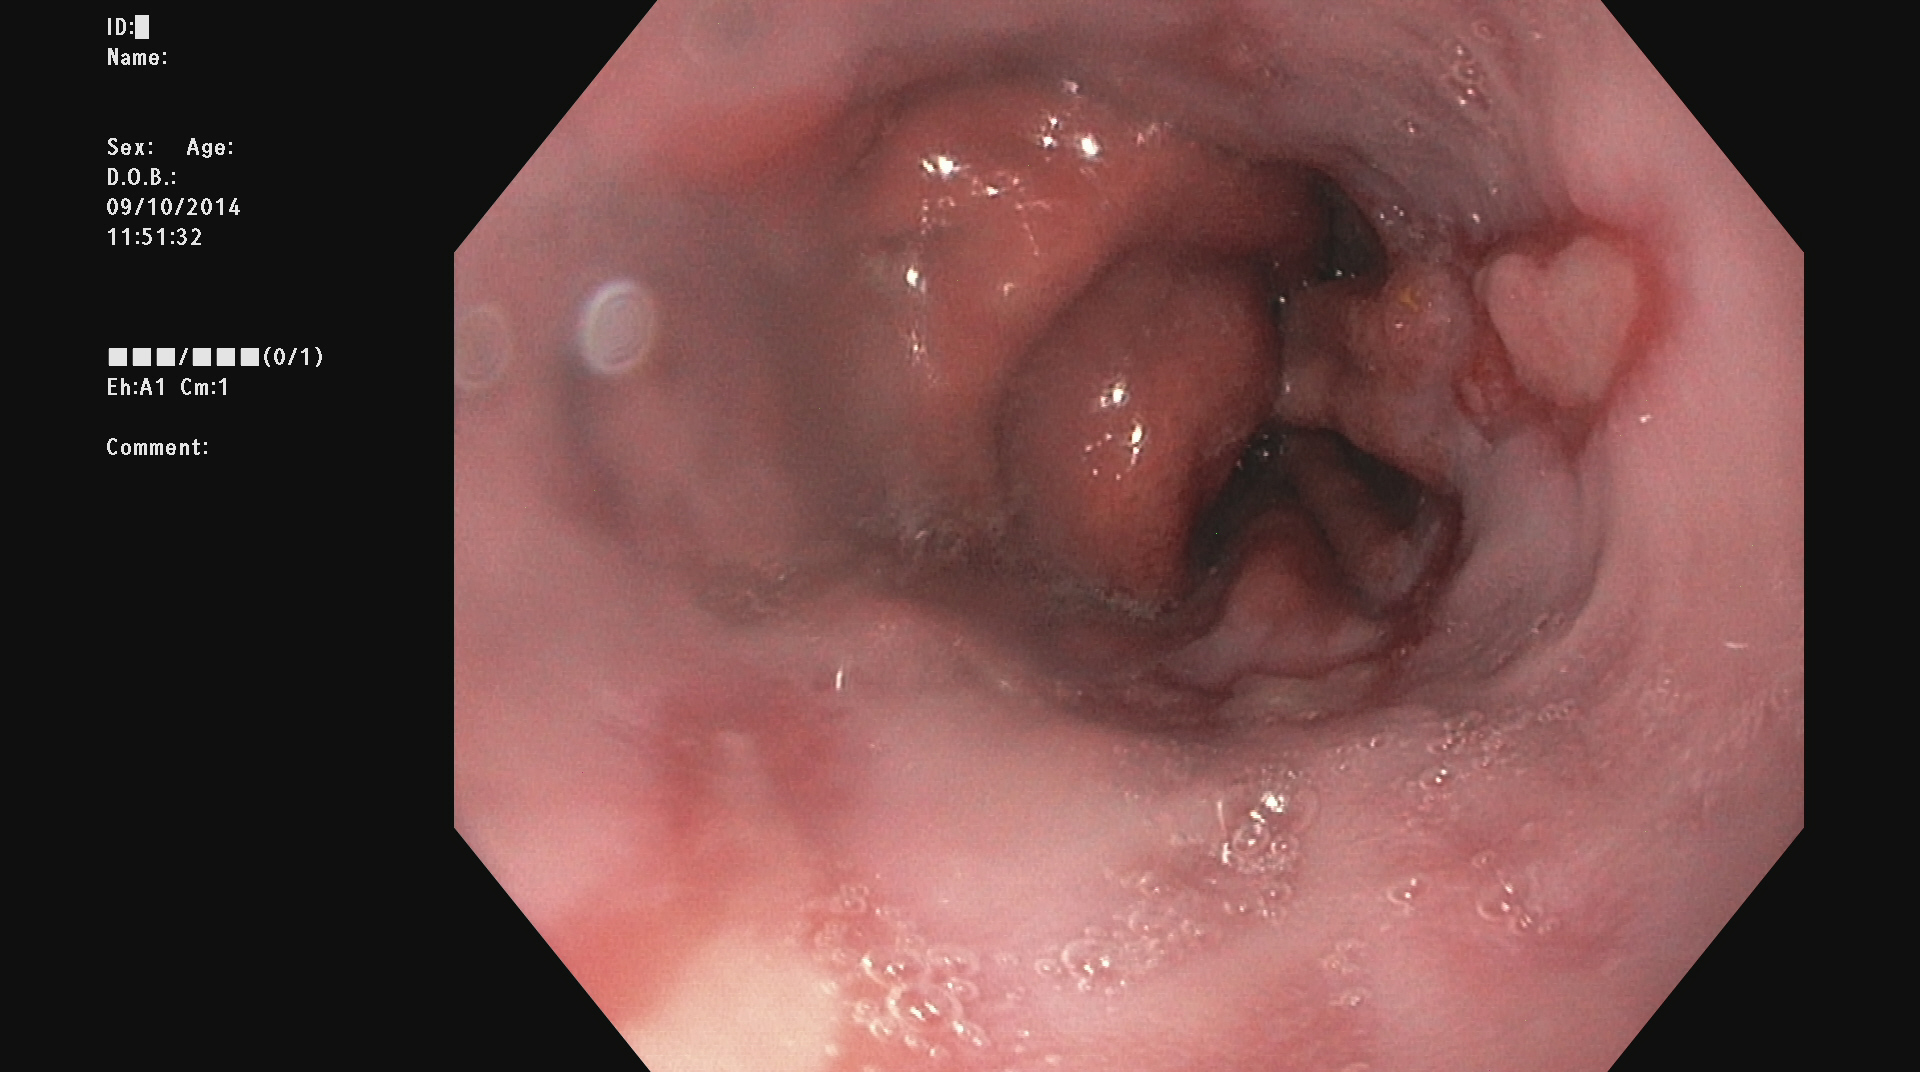
\includegraphics[height=5cm,width=\textwidth]{experiments/figures/leftframe.jpg}
         \caption{Example of an image with a large area without relevant medical information}
         \label{fig:LargeLeftBlack}
     \end{subfigure}
     \hfill
     \begin{subfigure}[b]{0.4\textwidth}
         \centering
         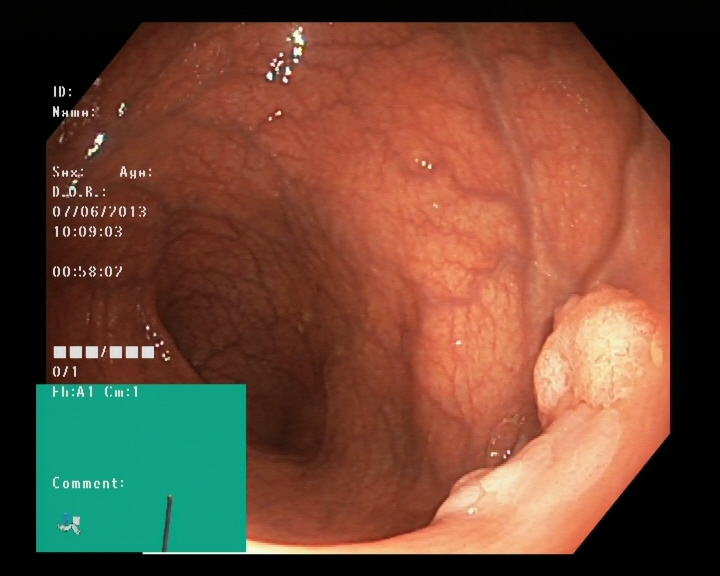
\includegraphics[height=6cm,width=\textwidth]{experiments/figures/greenframe.jpg}
         \caption{Example of an image with green square occluding the parts of the GI tract}
         \label{fig:GreenSquareOccluding}
     \end{subfigure}     
     \hfill
     \begin{subfigure}[b]{0.4\textwidth}
         \centering
         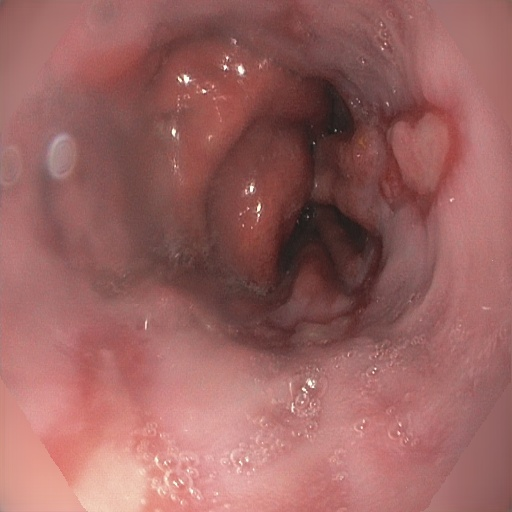
\includegraphics[width=\textwidth]{experiments/figures/noleftframe.jpg}
         \caption{The same image as in Figure \ref{fig:LargeLeftBlack} with the non-relevant information removed}
         \label{fig:LargeLeftBlackFIX}
     \end{subfigure}
     \hfill
     \begin{subfigure}[b]{0.4\textwidth}
         \centering
         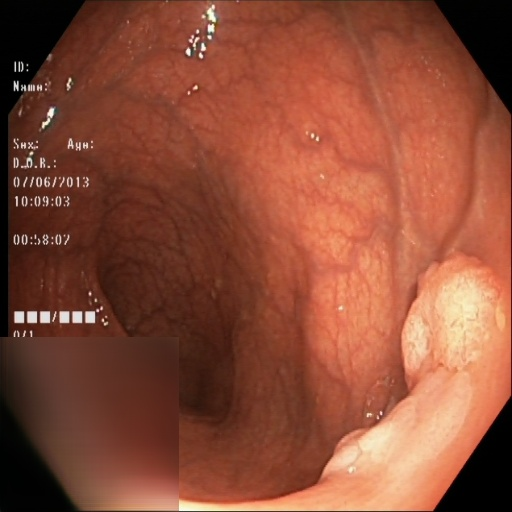
\includegraphics[width=\textwidth]{experiments/figures/nogreenframe.jpg}
         \caption{The same image as in Figure \ref{fig:GreenSquareOccluding} with the green square inpainted}
         \label{fig:GreenSquareOccludingFIX}
     \end{subfigure}
        \caption{Images where the troubling areas are removed before training}
        \label{fig:KvasirAnomaliesFIX}
\end{figure}



Compared to the CVC images we have images in the Kvasir set with this square and with additional text, both outside the image, and on top of the image.  

We propose different types of inpainting to prove or disprove our two hypothesises.

\subsection{Removing black corners}
The most straightforward experiment to conduct is to test how the removal of the black corners will affect the result.
As we propose in hypothesis \ref{hyp:a}, we believe that this masking can help with giving the classifier fewer areas with non-crucial information.

\todo{kvasir not presented yet}
The black edges around the images in the Kvasir set is also present in the CVC set. By removing the black corners around the image, we do not change Kvasir specific artefacts, but according to our first hypothesis, we believe we will get a higher classification accuracy since this removes areas with sparse information.






When classifying images during the testing stage, we need to take this mask in to account regarding the removal of black corners in the test set.
\begin{enumerate}
\item We can either do the same masking and inpainting on the test set. 
\item We can crop the image in a way that removes the black corners without inpainting.
\item We can forgo modifying the test data and just run the test set as is. 
\end{enumerate}


We tested method 1) in the paper ``Using preprocessing as a tool in medical image detection''\cite{26254}
The goal of this paper was related to hypothesis \ref{hyp:a} with the fact that we wanted to see how removing areas with sparse information affected the result of classification. 
In the experiments run within this paper, both the training set and test set were inpainted. 
Since the focus of this task was to classify a test set we had from beforehand correctly, we had the option to preprocess the test set in addition to the training set. This type is the same method proposed in method 1) and from the results, it showed minimal improvement. The lack of improvement is mainly not connected to the fact that we inpainted the test set, but the fact that the test set came from the same distribution as the training set.
Given that we, in the end, want to classify images from a live colonoscopy, we have decided to forgo the inpainting of the test set using method 1).
By not augmenting the test set the experiments are also suited to reflect a larger area of machine learning better.




Method number 2) was the proposal of cropping the images during evaluation.  Thambawita et al. did similar methods in the Mediaeval 2018 conference, but had also, the same cropping during training. In the paper ``The Medico-Task 2018: Disease Detection in the Gastrointestinal Tract using Global Features and Deep Learning''~\cite{26205} we can see that this method worked with great success. 
The operation of just cropping images is also multiple times as fast as inpainting images, so it is feasible for a live recording.  
The downside of cropping the images from the test set is the fact that we do not have control over what we remove from the data. Given that the test set might come from a completely different distribution, we might unwillingly remove information we desire to keep.

The last proposed method is not to augment the images during testing. This method, since we are not preprocessing the test data at all, the fastest when it comes to live classification. Without the augmentation, we risk getting a lower classification score, but we do not remove any data.


In this thesis we will use method number 3). 
We base this decision on that we want the final product to have the option to be used live and without the risk of losing data due to cropping.

Figure \ref{fig:CornerMask} shows the mask used to inpaint the corners.


 
\subsection{Removing green squares}
The next major area in question is the removal of the green squares located in the bottom left area of some of the medical images.  This area is a Kvasir specific artefact, and it is in 38\% of the images spanning five out of eight classes. 
By inpainting the lower left area we can see if our hypothesis \ref{hyp:b} is correct since here we are removing a dataset-specific feature that the network can use to determine classes. 
We have also chosen to inpaint every image, regardless of the green square is there or not. We do this so that the network can not ``learn'' that the pattern from the inpainted area correlates with the five classes with the green square, and hence defeating the purpose of the inpainting.


As with the black corners to be inpainted, we choose not to preprocess the test data, as this takes time, and should in theory not be necessary to get the right classification.
 
Figure \ref{fig:GreenMask} shows the mask used to inpaint the lower left corner.

\subsection{Removing both corners and the green square}
The last set we want to test is the combination of both inpainting the green square and the black corner. 
Here we hope that a combination of hypothesis \ref{hyp:a} and \ref{hyp:b} will give the strength of both methods without harmful interference. 

Figure \ref{fig:BothMask} shows the mask used to inpaint both areas at the same time.


\subsection{How to make the images (give better name)}
For each of the three areas we want to inpaint we need a training set we can use when training the autoencoder and GAN.

As we recall from chapter \ref{cha:Explaining_autoencoders} the autoencoder and GAN\footnote{It is necessary to mention that regular GANs does not use a ground truth when training, though our modified GAN do.} networks both use a ground truth when training.
When training we need images that are already inpainted as a reference point. We solve this by cropping the images as shown in figure \ref{fig:CornerMask}.
By removing the corners, we have an image where we know the whole ground truth, and the data is coming from the right distribution.
As figure \ref{fig:masks} shows, we use cropped versions when inpainting corners, and we use images without the green square when inpainting the left corner.

\begin{figure}
     \centering
     \begin{subfigure}[b]{0.3\textwidth}
         \centering
         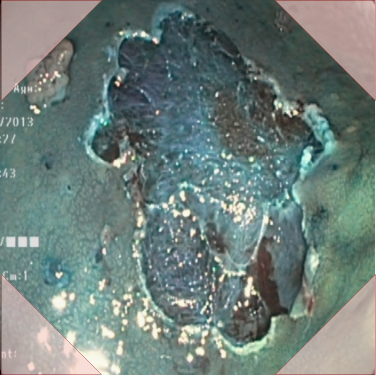
\includegraphics[width=\textwidth]{methodology/figures/cornermask.png}
         \caption{Green area shows the area masked in the first of the generated datasets}
         \label{fig:CornerMask}
     \end{subfigure}
     \hfill
     \begin{subfigure}[b]{0.3\textwidth}
         \centering
         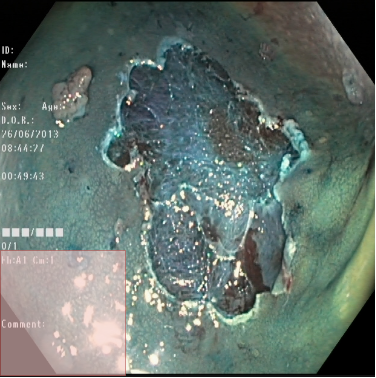
\includegraphics[width=\textwidth]{methodology/figures/greenmask.png}
         \caption{Green area shows the area masked by the second of the datasets}
         \label{fig:GreenMask}
     \end{subfigure}     
     \hfill
     \begin{subfigure}[b]{0.3\textwidth}
         \centering
         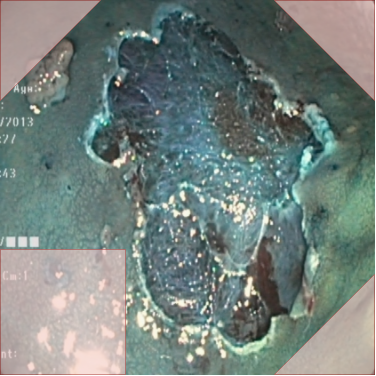
\includegraphics[width=\textwidth]{methodology/figures/bothmask.png}
         \caption{Green area shows the area masked by the third of the datasets}
         \label{fig:BothMask}
     \end{subfigure}
     \caption{All three mask types used in this thesis, and associated images used during training. At dataset in}
     \label{fig:masks}
\end{figure}


\section{Design of the transfer learning experiments}
The second part of the thesis is to check the success of the inpainted models. 
We use a convolutional neural net to achieve this.


\begin{figure}[h]
        \centering
        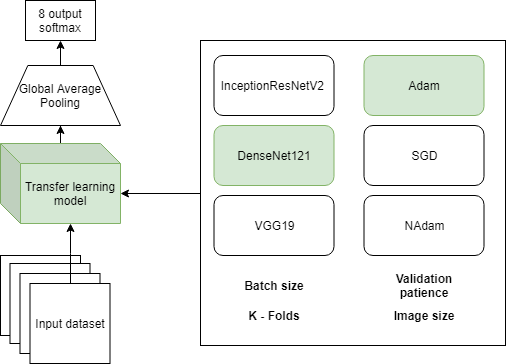
\includegraphics[scale=0.5]{experiments/figures/model.png}
        \caption{ The model we use for classifying with the most important options for the learning process. }
    \label{fig:KTLmodel}
\end{figure}

 
\section{Describe code}
We have, at this point, gone through the goal of our thesis, and shown how we want our result to be generated and evaluated in practice. 
We will now go more in-depth into the two networks used for generating the new datasets and go in-depth into the model we use for classification.


\subsection{autoencoder}
The autoencoder we used to generate the datasets used in this thesis bears a resemblance to the standard autoencoder proposed in chapter \ref{cha:Explaining_autoencoders}.

\paragraph{loss, optimiser}
To get the autoencoder to give the best result, we have chosen to use the mean square error loss\ref{MSE_form} and the Adam\cite{adam} optimiser.
The mean square error was a logical choice since we already have the ground truth and we only want to recreate the inpainted area based on what used to be there before the masking.
The Adam optimiser was chosen by the widespread usage in machine learning, coupled with the fact that it works well with sparse gradiens.

\paragraph{encoder}
The input to the autoencoder were the masked images at $256 \times 256$px to compress the information in the ecoder we imply used convolutions with a stride of 2.

Input(InputLayer)         (None, 256, 256, 3)      0 \\
conv2d(Conv2D)            (None, 64, 64, 32)       51232    \\ 
conv2d(Conv2D)            (None, 32, 32, 64)       204864    \\
conv2d(Conv2D)            (None, 16, 16, 128)      204928\\  \todo{do i keep this???}

\paragraph{decoder}
After 

dropout (Dropout)          (None, 16, 16, 128)       0         \\
(UpSampling2 (None, 32, 32, 128)       0         \\
conv2d (Conv2D)            (None, 32, 32, 256)       7373056   \\
(UpSampling2 (None, 64, 64, 256)       0    \\     
conv2d (Conv2D)            (None, 64, 64, 128)       1605760   \\
(UpSampling2 (None, 128, 128, 128)     0       \\ 
conv2d (Conv2D)            (None, 128, 128, 32)      102432    \\
(UpSampling2 (None, 256, 256, 32)      0       \\  
conv2d (Conv2D)            (None, 256, 256, 3)       867 \\


To describe the model we will look at the example where we try to inpaint the green square in the image, and nothing else.

To train the autoencoder for inpainting, we divide the dataset in two, first images with the green square and images without the green square. We discard the images with the green square since they are not viable for training. 
The resulting dataset will only contain images without green sources.

\begin{figure*}[]
\centering
\begin{subfigure}[b]{0.45\textwidth}
    \centering
    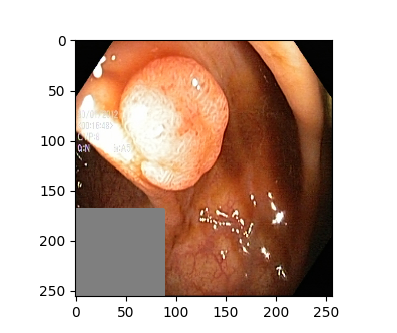
\includegraphics[width=\textwidth]{methodology/figures/masked_img.png}
    \caption{Image the autoencoder receives as an input }    
    \label{fig:AErec}
\end{subfigure}
\hfill
\begin{subfigure}[b]{0.49\textwidth}  
    \centering 
    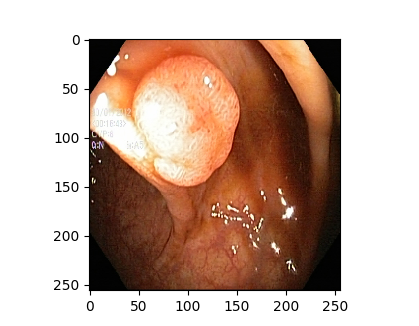
\includegraphics[width=\textwidth]{methodology/figures/whole_img.png}
    \caption[Hate to be this guy]%
    {{\small The missing part the autoencoder tries to replicate}}    
    \label{fig:AErep}
\end{subfigure}
\caption{A standard image taken in by the autoencoder} 
\label{fig:AEmasks}
\end{figure*}

The next step before training is to cut the images according to the mask provided. Figure \ref{fig:AErec} shows what the finished masking looks like, and \ref{fig:AErep} shows what we want to achieve after training.

We feed \ref{fig:AErep} into the autoencoder consisting of convolutional layers, leakyReLu layers, and a tanh layer.
\todo{more}
\todo{remember to talk about loss}


\subsection{Generative adversarial network}
The gan used the same generator discriminator elements as the Goodfellow gan, but does not take in noise\todo{the best version does}


\subsection{Transfer learning classifier}
The dataset we are making with our generators needs to be classified. 

The classifier we use is based on the idea of reusing networks we already know apply well to the real world.
We have made a classifier that, by default, use one of the pretrained networks provided by the Keras framework.

\begin{table}[h]
\caption{Datasets provided by keras}
\begin{center}
\small
\begin{tabular}{llllll}
\toprule
\multicolumn{1}{c}
{Model}             & Size   & Top-1 Accuracy & Top-5 Acc & Parameters  & Depth \\
\midrule
Xception          & 88 MB  & 0.790          & 0.945          & 22,910,480  & 126   \\
VGG16             & 528 MB & 0.713          & 0.901          & 138,357,544 & 23    \\
VGG19             & 549 MB & 0.713          & 0.900          & 143,667,240 & 26    \\
ResNet50          & 98 MB  & 0.749          & 0.921          & 25,636,712  & -     \\
ResNet101         & 171 MB & 0.764          & 0.928          & 44,707,176  & -     \\
ResNet152         & 232 MB & 0.766          & 0.931          & 60,419,944  & -     \\
ResNet50V2        & 98 MB  & 0.760          & 0.930          & 25,613,800  & -     \\
ResNet101V2       & 171 MB & 0.772          & 0.938          & 44,675,560  & -     \\
ResNet152V2       & 232 MB & 0.780          & 0.942          & 60,380,648  & -     \\
ResNeXt50         & 96 MB  & 0.777          & 0.938          & 25,097,128  & -     \\
ResNeXt101        & 170 MB & 0.787          & 0.943          & 44,315,560  & -     \\
InceptionV3       & 92 MB  & 0.779          & 0.937          & 23,851,784  & 159   \\
InceptionResNetV2 & 215 MB & 0.803          & 0.953          & 55,873,736  & 572   \\
MobileNet         & 16 MB  & 0.704          & 0.895          & 4,253,864   & 88    \\
MobileNetV2       & 14 MB  & 0.713          & 0.901          & 3,538,984   & 88    \\
DenseNet121       & 33 MB  & 0.750          & 0.923          & 8,062,504   & 121   \\
DenseNet169       & 57 MB  & 0.762          & 0.932          & 14,307,880  & 169   \\
DenseNet201       & 80 MB  & 0.773          & 0.936          & 20,242,984  & 201   \\
NASNetMobile      & 23 MB  & 0.744          & 0.919          & 5,326,716   & -     \\
NASNetLarge       & 343 MB & 0.825          & 0.960          & 88,949,818  & -        \\   
\bottomrule
\end{tabular}
\end{center}
\label{tab:Kaeras_app}
\end{table}

Table \ref{tab:Kaeras_app} shows the pretrained networks available to load in the Keras framework. 
When training we did some extra steps at the end, namely added global average pooling and a fully connected layer with the desired number of outputs (usually eight classes, and eight outputs)




\section{Describe project}
Here i am going to explain the projects
\section{Summary}
At this point, we have described the reasoning behind using python, tensorflow and Keras for our machine learning. 
After this we looked into the filters used for training our models, and what type of preprocessing we wanted to do in addition to the inpainting. We looked at the advantages and disadvantages of preprocessing the Trest data, as opposed to just preprocessing the training data.

We then went more in-depth into how the three main programs were built up, and how they differ from their original sources.
First, we looked at the preprocessing methods, AE and GAN. We looked at how they learned from the samples, and we went more in-depth talking about the crucial layers for each model.

At last, we ended up giving a summary of the project as a whole, following a the Kvasir dataset from its original source into the generation of the six new datasets, and how each one of them was classified with all the different parameters to show the dataset-specific rate of success.

 
